{
     \lstset{
        numbers=none,
        numberstyle=\scriptsize,
        language=[LaTeX]TeX,
        commentstyle=\color{white},
        keywordstyle=\color{blue}
 }
%   这是为了插入LaTeX代码

%  正文章节从下面开始
\chapter{模板使用}
\songti\xiaosi
\begin{spacing}{1.5}

\noindent \textbf{Q.Y. Fang [2018-3-10]:}

本项目为非官方的南京理工大学本科生毕业论文(理工类)\LaTeX 模板,考虑目前没人制作本科生毕设模板,小白一枚的本人自告奋勇地制作了该模板,基本上符合2017年南京理工本科生毕业论文官方word模板格式,如有问题之处欢迎大家向我提出。

此外本人在此声明:目前只有我自己使用此模板完成过毕业设计(注:我用的理工类),任何人使用本模板进行该模板排版均属于自愿行为,如发生任何问题,本人概不负责。
\vspace{1ex}

\noindent \textbf{J.X. Zhang [2019-6-7]:}

基于Fang学长的南京理工大学本科生毕业论文(理工类)\LaTeX 模板进行修改,使其基本符合2019年官方word模板格式,在一些细节方面和官方模板仍然有所出入,例如还有封面日期的字体、一级标题文字和数字之间的距离、页眉的加粗等。这些细节都不容易被发现,本人使用此模板撰写的毕业论文在提交、查重、审阅过程中都未出现问题。尽管如此,本人还是在此声明:任何人使用本模板进行该模板排版均属于自愿行为,如发生任何问题,本人概不负责。

感谢各位学长的贡献。本人才疏学浅,模板尚有改进空间,望后辈继续努力。

\section{图片使用}
为了方便于管理,所有的图片均放在figure文件下。在输入图片名称时,需要在前面添加一个相当于路径的语句“figure//”,以下文本框中给出一个图片插入的例子。在某些情况下,如果不想让图片浮动把\fbox{[htb]}选项改成\fbox{[H]},H为强制禁止浮动,但会拉宽段间距和公式与正文之间距离,结合自己需求进行调整。这里已经把图片标题的格式和前后间距都已经设置,可以直接使用“$\setminus$caption”即可。
\vspace{-4ex}
\begin{lstlisting}
\begin{figure}[htb]
  \centering
  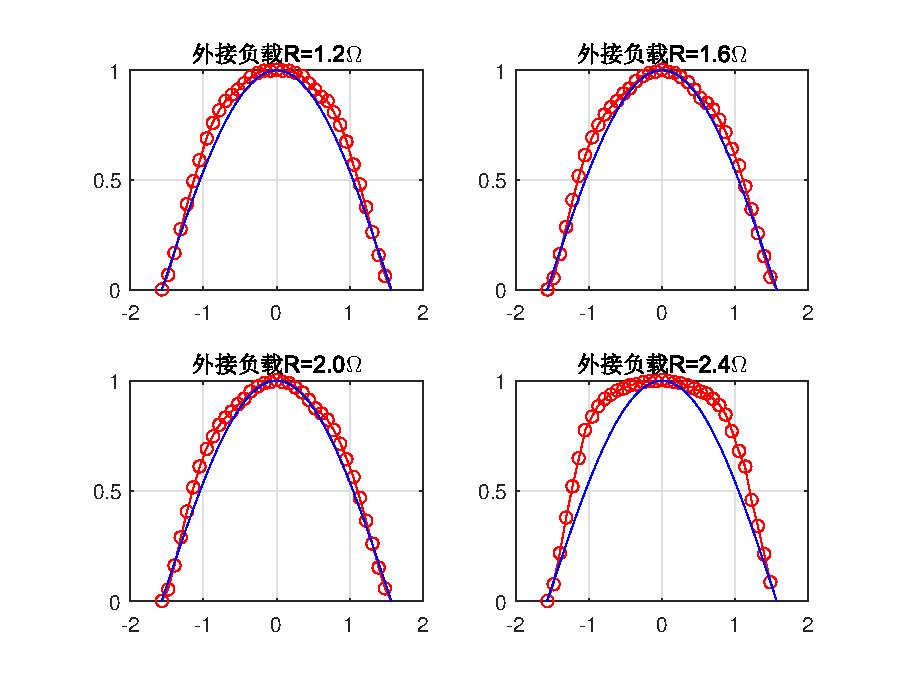
\includegraphics[width=0.65\textwidth]{figure//fig_calculate}
  \caption{SampleFigure1}\label{samplefigure1}
\end{figure}
\end{lstlisting}
\vspace{-0.5ex}

图\ref{samplefigure1} 为以上程序得到图片效果。

若要在页面中并列放置两或者更多张图片,请使用\fbox{$\setminus$begin\{minipage\}}环境,并且使最左侧和最右侧的图片尽量与文字的边缘对齐。考虑到对称性,图片可能需要裁剪来去除部分边缘,通过设置trim属性可以进行裁剪,其四个值按照顺序分别为左侧、下侧、右侧和上侧的裁减量。效果如图\ref{samplefigure2} 和\ref{samplefigure3} 所示。
\newpage
\vspace{-4ex}
\begin{lstlisting}
\begin{figure}[htb]
	\begin{minipage}[b]{0.5\textwidth}
		\flushleft
		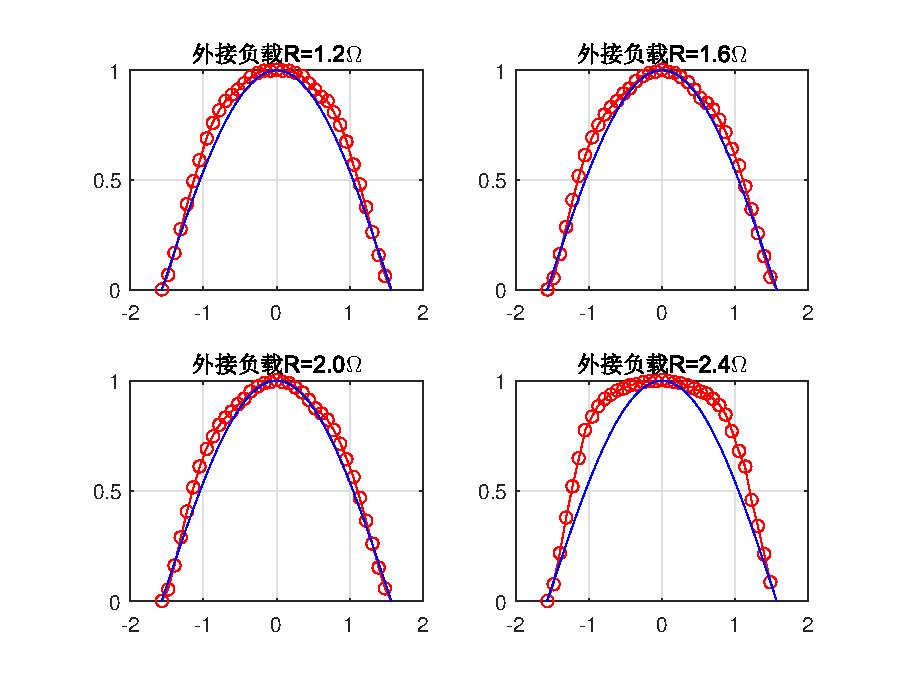
\includegraphics[width=\textwidth,trim=0 20 0 0,clip]{figure//fig_calculate}
		\caption{SampleFigure2}\label{samplefigure2}
	\end{minipage}
	\hfill
	\begin{minipage}[b]{0.5\textwidth}
		\flushright
		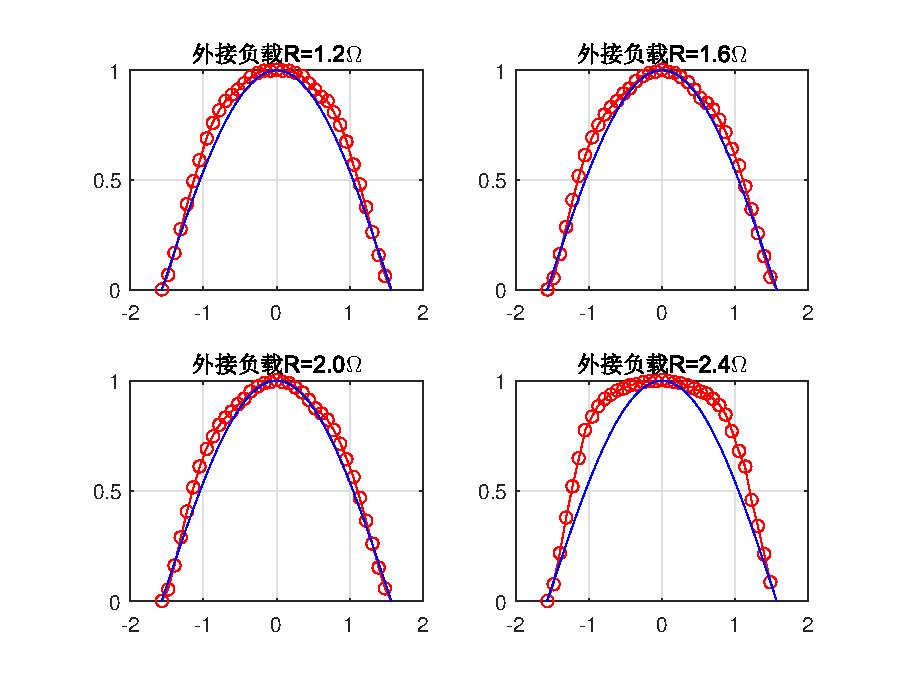
\includegraphics[width=\textwidth,trim=0 20 0 0,clip]{figure//fig_calculate}
		\caption{SampleFigure3}\label{samplefigure3}
	\end{minipage}
\end{figure}
\end{lstlisting}
\vspace{1ex}

\begin{figure}[htbp]
	\centering
	% Requires \usepackage{graphicx}
	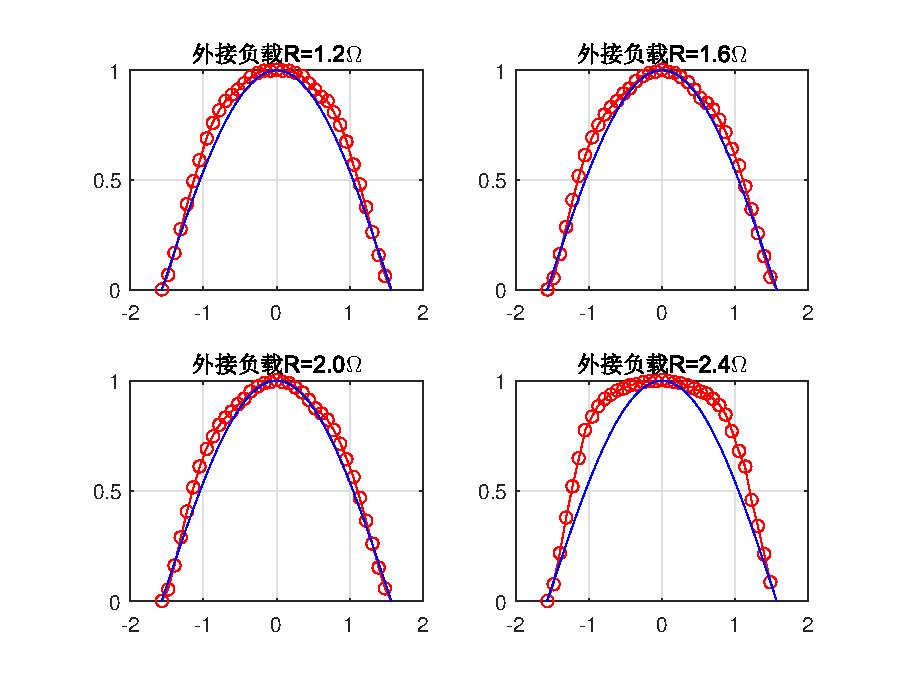
\includegraphics[width=0.6\textwidth, trim=0 20 0 0,clip]{figure//fig_calculate}
	\caption{SampleFigure1}\label{samplefigure1}
\end{figure}

\begin{figure}[htb]
	\begin{minipage}[b]{0.5\textwidth}
		\flushleft
		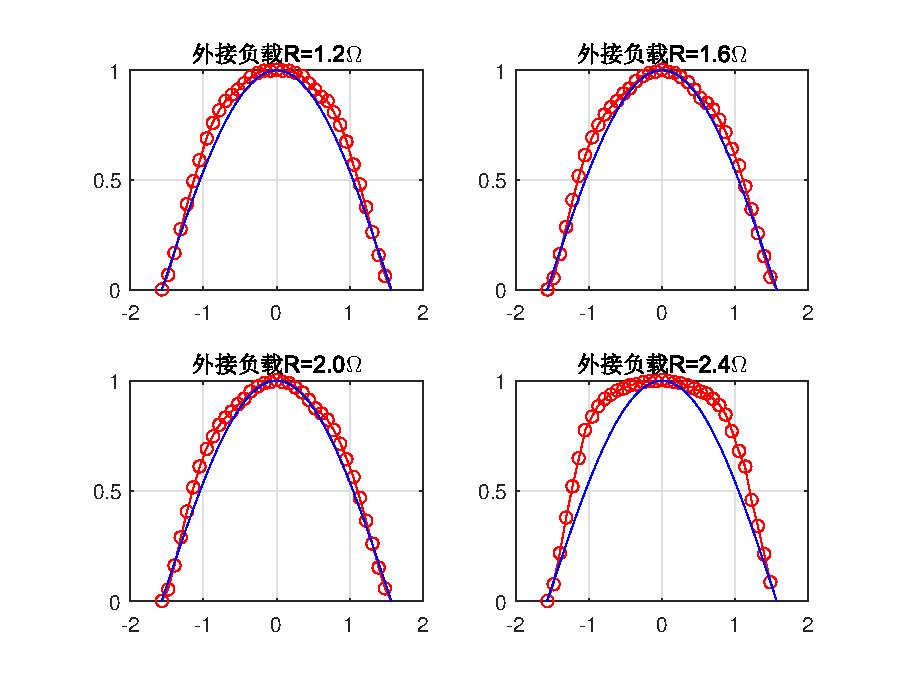
\includegraphics[width=\textwidth,trim=35 20 20 0,clip]{figure//fig_calculate}
		\caption{SampleFigure2}\label{samplefigure2}
	\end{minipage}
	\hfill
	\begin{minipage}[b]{0.5\textwidth}
		\flushright
		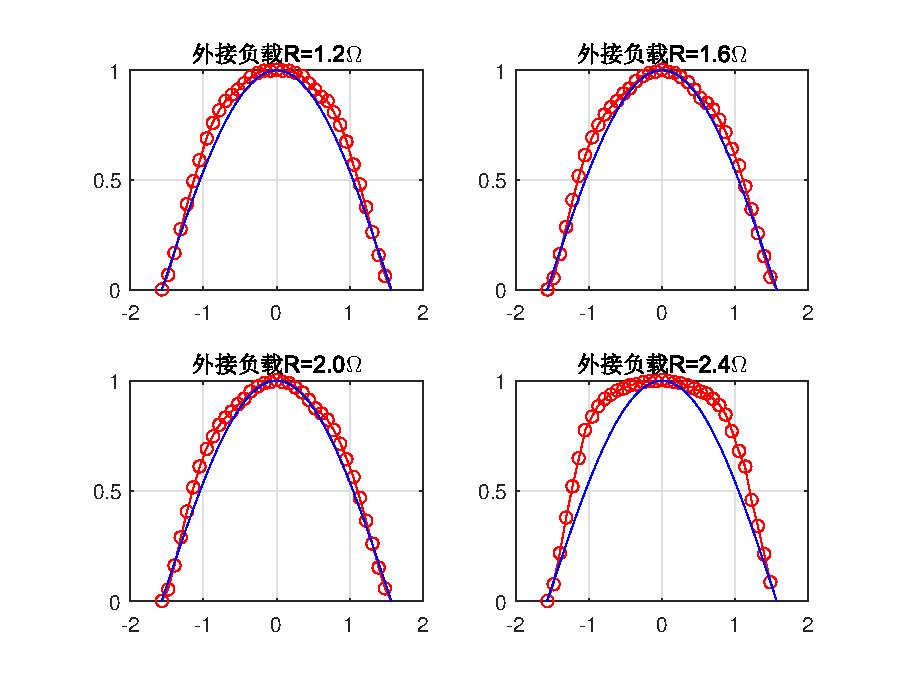
\includegraphics[width=\textwidth,trim=20 20 35 0,clip]{figure//fig_calculate}
		\caption{SampleFigure3}\label{samplefigure3}
	\end{minipage}
\end{figure}

\newpage
\section{表格使用}
由于学校要求三线表格,自己在制作时需要注意该点,表格中的文字应该为五号宋体,结合两点要求,文本框中给出一个表格的范例。为了区分和图片的标题命名,在使用表格时使用“$\setminus$topcaption”,表格标题的格式和前后间距都已经设置。

\vspace{-4ex}
\begin{lstlisting}
{\zihao{5}\songti
\begin{table}[htb]
\begin{center}
\topcaption{SampleTable}\label{sampeltable}
\begin{tabular}{m{3cm} m{2cm} m{2cm} m{2cm}}
  \hline
  Project & A & B & C\\
  \hline
  ProjectOne   & a1 & b1 & c1 \\
  ProjectTwo   & a2 & b2 & c2 \\
  ProjectThree & a3 & b3 & c3 \\
  ProjectFour  & a4 & b4 & c4 \\
  ProjectFive  & a5 & b5 & c5 \\
  \hline
\end{tabular}
\end{center}
\end{table}}
\end{lstlisting}
\vspace{-2ex}

下表\ref{sampeltable}是一个表格示例。

{\wuhao\songti
\begin{table}[htb]
\begin{center}
\topcaption{SampleTable}\label{sampeltable}
\begin{tabular}{m{3cm} m{2cm} m{2cm} m{2cm}}
  \hline
  Project & A & B & C\\
  \hline
  ProjectOne& a1 & b1 & c1 \\
  ProjectTwo & a2 & b2 & c2 \\
  ProjectThree & a3 & b3 & c3 \\
  ProjectFour& a4 & b4 & c4 \\
  ProjectFive & a5& b5 & c5 \\
  \hline
\end{tabular}
\end{center}
\end{table}}

考虑到使用该模板大部分是和我一样的小白,这里做一个小提示,毕业设计由于图表都比较多,如果在正文中用到图1.1、表1.1、 式1.1 等词,最好在正文使用\fbox{图$\setminus$ref\{samplefigure\}}、\fbox{表$\setminus$ref\{sampeltable\}}对图表的标号确定。前提是figure和table已经用\fbox{$\setminus$label\{samplefigure\}}、\fbox{$\setminus$label\{sampeltable\}} 进行标记。每个图标和公式的标记应该是唯一的,重复会出现警告。

上述方法是为了避免在写作过程,突然需要前面的图表和公式进行增添或删减,不再需要手动改图标的标号。

\section{公式使用}
对于公式使用\fbox{$\setminus$begin\{equation\}}环境,如果有多行公式可以使用\fbox{$\setminus$begin\{split\}}环境,符号“\&”为各行公式对齐的位置。

公式和上下文之间默认间距较大,可使用\fbox{$\setminus$equationskip}和\fbox{$\setminus$equationskipfrac}命令来缩小间距,前者适用于简单的单行公式,后者适用于带有分式、矩阵的单行公式或者多行公式。

如果需要对公式中的字母进行注释,并且注释较多,这里推荐一种方法,可以使用表格的环境,表格为2列,第一列字母靠右,第二列解释靠左,如\fbox{$\setminus$begin\{tabular\}\{r@\{---\}l\}}。 
下面文本框中给出了一个多行公式以及注释的示例。

\vspace{-4ex}
\begin{lstlisting}
\begin{equation}\label{SampleEquation}
  \equationskipfrac
  \begin{split}
  \bm{x_}k&=\bm{\Phi}_{k,k-1}\bm{x}_{k-1}+\bm{\Gamma}_{k-1}\bm{w}_{k-1}\\
  \bm{z}_k&=\bm{H}_k\bm{x}_k+\bm{v}_k
  \end{split}
\end{equation}
\begin{tabular}{r@{---}l}
  $\bm{x}_k$  & The state variable of the $k^{th}$ step;\\
  $\bm{z}_k$  & The observation of the $k^{th}$ step; \\
  $\bm{\Phi}_{k,k-1}$ & The transition matrix of the $(k-1)^{th}$ to $k^{th}$ step; \\
  $\bm{\Gamma}_{k-1}$  & The measurement noise driving matrix of the $k^{th}$ step; \\
  $\bm{v}_k$ & The measurement noise of the $k^{th}$ step,$\bm{v_k}\sim N(0,\bm{R}_k)$.
\end{tabular}
\end{lstlisting}
\vspace{-1ex}

下式\ref{sampeltable}和注释为上面程序的效果,数学符号可以自行百度,或者在这\url{http://www.mohu.org/info/symbols/symbols.htm}上面寻找,几乎包含了基本上要用的数学符号。
\begin{equation}\label{SampleEquation}
  \equationskipfrac
  \begin{split}
  \bm{x_}k&=\bm{\Phi}_{k,k-1}\bm{x}_{k-1}+\bm{\Gamma}_{k-1}\bm{w}_{k-1}\\
  \bm{z}_k&=\bm{H}_k\bm{x}_k+\bm{v}_k
  \end{split}
\end{equation}
式中:

\begin{tabular}{r@{---}l}
  $\bm{x}_k$  & The state variable of the $k^{th}$ step;\\
  $\bm{z}_k$  & The observation of the $k^{th}$ step; \\
  $\bm{\Phi}_{k,k-1}$ & The transition matrix of the $(k-1)^{th}$ to $k^{th}$ step; \\
  $\bm{\Gamma}_{k-1}$  & The measurement noise driving matrix of the $k^{th}$ step; \\
  %$\bm{H}_k$  & The measurement matrix of the $k^{th}$ step;\\
  %$\bm{w}_{k-1}$ & The systematic noise of the $(k-1)^{th}$ step ,$\bm{w}_{k-1}\sim N(0,\bm{Q}_{k-1})$;\\
  $\bm{v}_k$ & The measurement noise of the $k^{th}$ step,$\bm{v_k}\sim N(0,\bm{R}_k)$.
\end{tabular}

\newpage
\section{枚举格式}
官方模板未对枚举格式做出规定。但为了方便使用,本模板参考了大部分中文期刊的排版,对枚举格式做出了设置。枚举使用\fbox{$\setminus$begin\{enumerate\}}环境,编号为带有括号的数字,每个item的首行开头缩进两个字符,其余行不缩进。考虑到美观,不建议在item内部进行分段。示例如下:

\vspace{-4ex}
\begin{lstlisting}
\begin{enumerate}
	\item 内容一,内容一,内容一,内容一……
	\item 内容二,内容二,内容二,内容二……
	\item 内容三,内容三,内容三,内容三……
\end{enumerate}
\end{lstlisting}
\vspace{-1ex}

\begin{enumerate}
	\item 内容一,内容一,内容一,内容一,内容一,内容一,内容一,内容一,内容一,内容一,内容一,内容一,内容一。
	\item 内容二,内容二,内容二,内容二,内容二,内容二,内容二,内容二,内容二,内容二,内容二,内容二,内容二。
	\item 内容三,内容三,内容三,内容三,内容三,内容三,内容三,内容三,内容三,内容三,内容三,内容三,内容三。
\end{enumerate}

\section{参考文献}
参考文献在ThesisReference中\fbox{$\setminus$begin\{thebibliography\}}环境中进行填写,具体格式规范查阅参考文献标注国家标准GB/T~7714——2015。按照官方模板的要求,编号和参考文献内容分别左对齐。本模板使用box对编号的位置进行约束\fbox{$\setminus$makebox[1.5em][l]\{[\#1]\}},设定宽度为1.5em,该值适用于一位和两位的编号,若编号达到三位数,则需要自行调整宽度。

模板参考文献使用下面文本框中方法,该方法比较业余,不便于大量参考文献的管理,并且需要手动输入书目信息。专业的方法是使用BibTeX,使用方法自行百度,BibTeX可以在Google scholar、百度学术上直接导入。

\vspace{-4ex}
\begin{lstlisting}
\begin{thebibliography}
\bibitem author,article, year, vol,
\end{thebibliography}
\end{lstlisting}

正文需要引用文献,使用\fbox{$\setminus$cite\{\}}即可。

\section{代码插入}
考虑到大多数同学的代码应该是MATLAB,在ThesisAppendix文件中将语言设置m语言,可以根据自身需要进行改变。网上的Mcode包编译效果非常不错,这里就直接拿来,做一回拿来主义。

Mcode包效果在附录B MATLAB Code中看到,其能较好地还原MATLAB本身的编程风格。程序代码需放到\fbox{$\setminus$begin\{lstlisting\}}环境中。

由于某些未知的原因,如果\fbox{$\setminus$begin\{lstlisting\}}环境跨页,可能会导致页眉出现乱码,所以使用时请注意代码的长度和放置的位置。

建议在\fbox{$\setminus$begin\{lstlisting\}}环境开始前用\fbox{$\setminus$vspace\{-4ex\}},结束后用\fbox{$\setminus$vspace\{-1.5ex\}}来减少代码和上下文之间的距离,具体数值需要按照实际情况调整。

\end{spacing}
}